%!TEX root = ../../main.tex

\chapter{Bilder}

Lorem ipsum dolor sit amet, consetetur sadipscing elitr, sed diam nonumy eirmod tempor invidunt 
\section{Ein Bild ganz breit} 
Verweis auf das Beispielbild \ref{fig:example}

\begin{figure}[htbp]
 \centering
 \includegraphics[width=\linewidth]{content/images/03_3_example}
 \caption{Beispielbild}
 \label{fig:example}
\end{figure}

\section{Zwei Bilder nebeneinander} 

\begin{figure}
\subfigure[Promises]{\label{fig:promises}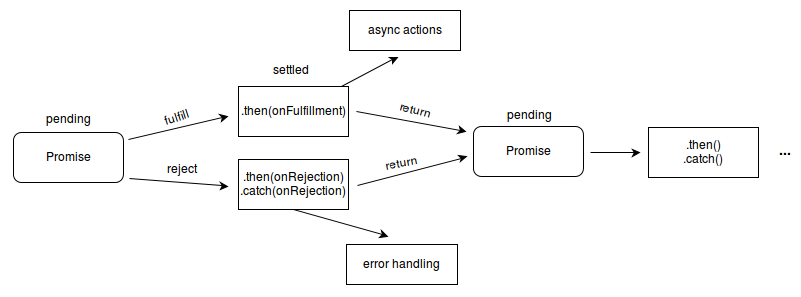
\includegraphics[width=0.50\textwidth]{content/images/03_3_promises}}\hfill
\subfigure[MVC Pattern]{\label{fig:mvc}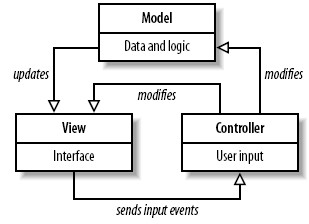
\includegraphics[width=0.50\textwidth]{content/images/03_3_mvc}}
\caption{Beispiel mit zwei Bildern nebeneinander}
\end{figure}
